\begin{figure*}[htbp]
    \centering
    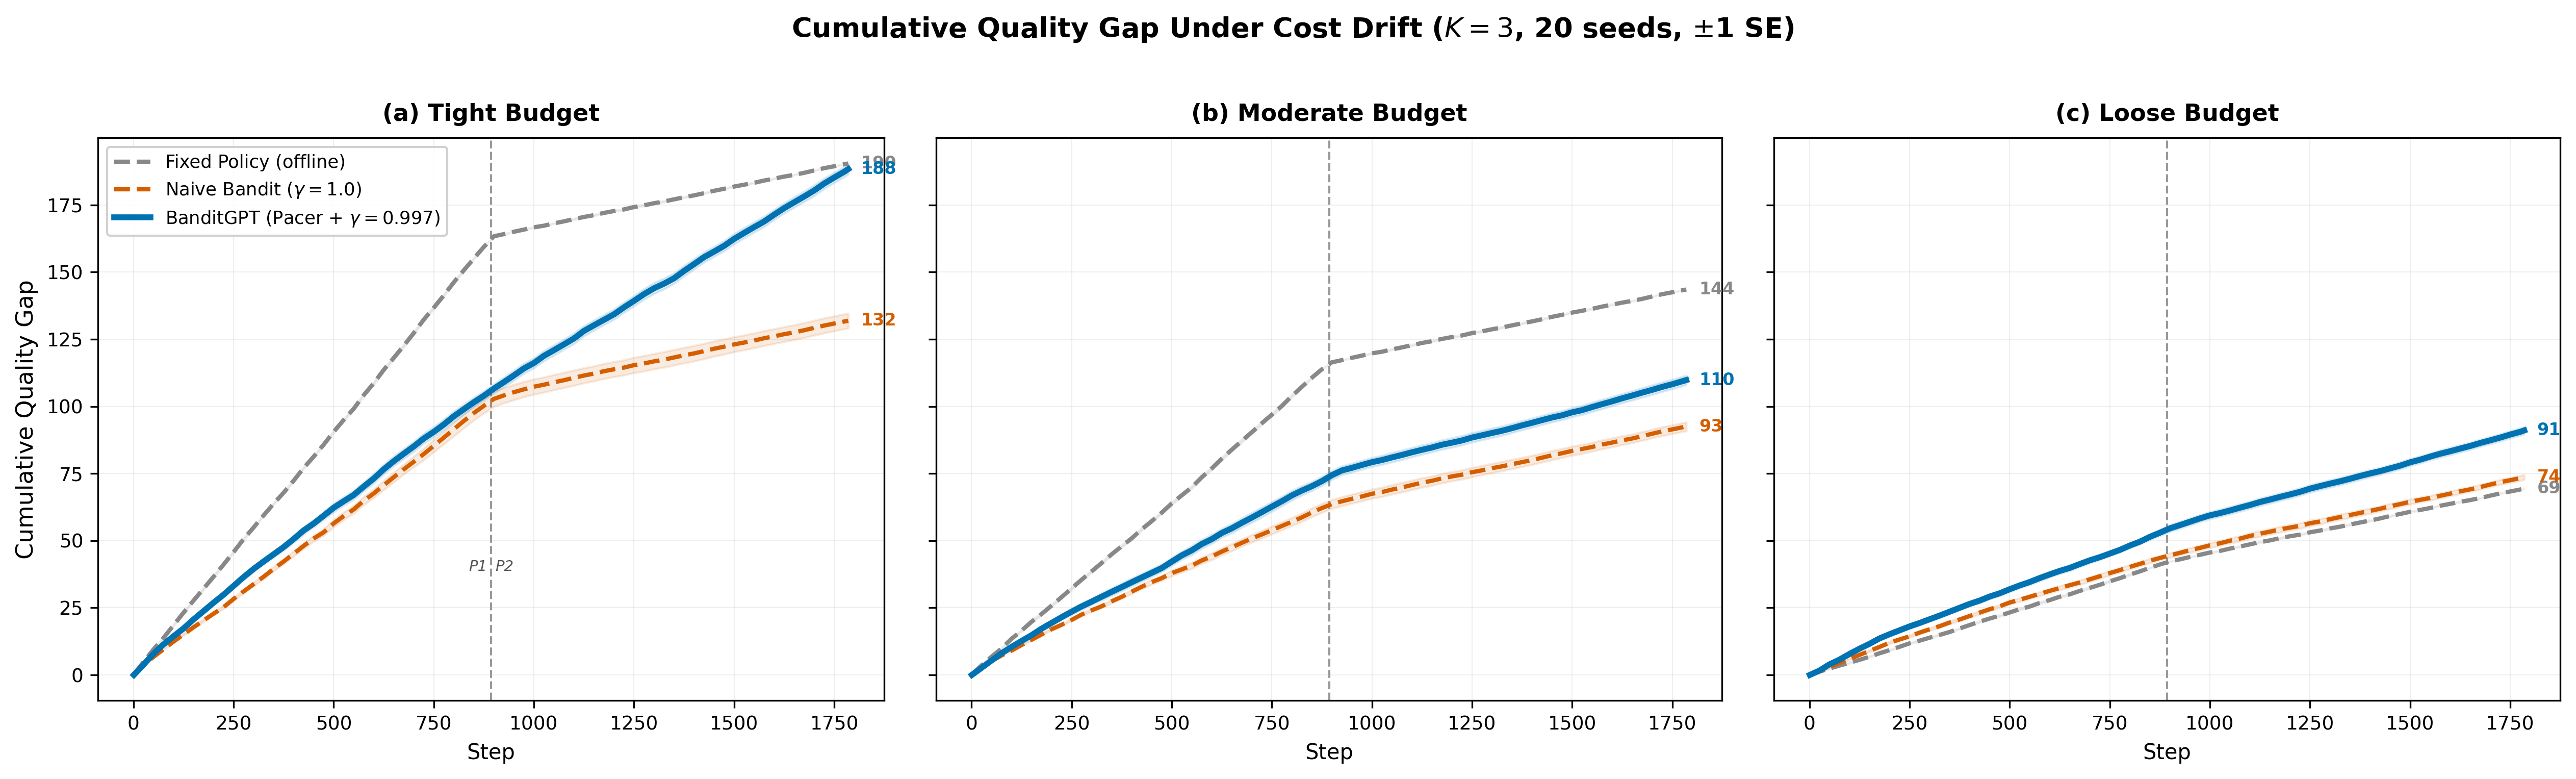
\includegraphics[width=\linewidth]{../experiments/03_budget_plus_drift/results/cumulative_quality_gap.pdf}
    \caption{Cumulative quality gap under cost drift at three budget
    levels ($K{=}3$; 20~seeds, $\pm$1\,SE shading).
    %
    The quality gap measures the cumulative difference between the
    unconstrained per-round best reward and the chosen arm's reward:
    $G_T = \sum_{t=1}^T [\max_a r_{a,t} - r_{a_t,t}]$.
    Lower is better.  The dashed vertical line marks the Phase~1/Phase~2
    boundary (Gemini price drop at step~893).
    %
    \textbf{Fixed Policy} (gray, dashed): frozen warmup priors with a
    matched static cost penalty.  Cannot update reward estimates, so the
    quality gap grows linearly in both phases.
    %
    \textbf{Naive Bandit} (orange, dashed): LinUCB with $\gamma{=}1.0$
    and the same static cost penalty.  Online learning reduces the
    quality gap in Phase~1, but infinite memory causes slow adaptation
    to the cost shift---Phase~1 inertia dilutes the Phase~2 signal.
    %
    \textbf{BanditGPT} (blue, solid): warmup priors with geometric
    forgetting ($\gamma{=}0.997$) and the primal-dual BudgetPacer.
    Adapts most rapidly to the price drop: the quality gap flattens
    in Phase~2 as the pacer detects declining costs, reduces
    $\lambda_t$, and routes more traffic to the now-cheap Gemini.
    %
    At moderate and loose budgets, BanditGPT achieves the lowest
    final quality gap.  At tight budget, BanditGPT's quality gap is
    comparable to the Fixed Policy because the stringent budget
    suppresses exploration of expensive arms (exploration starvation;
    see Section~\ref{sec:budget_drift}).
    }
    \label{fig:exp03_quality_gap}
\end{figure*}
